	\begin{figure}[H]
		\centering
 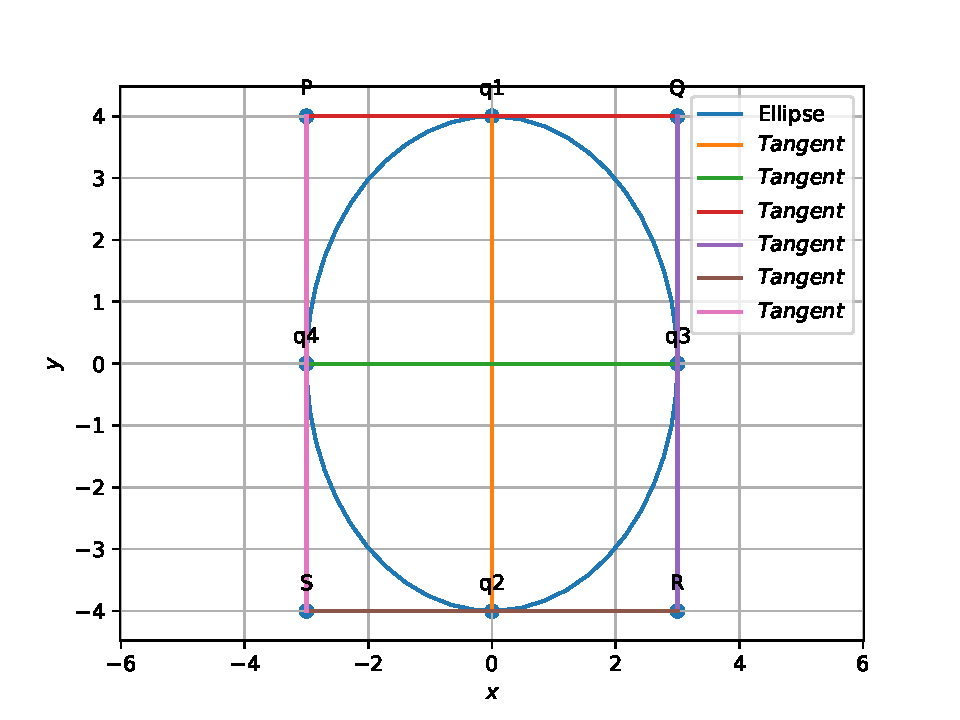
\includegraphics[width=0.75\columnwidth]{chapters/12/6/3/13/figs/conic_1.pdf}
		\caption{}
		\label{fig:12/6/3/13}
  	\end{figure}
The parameters of the given conic are
\begin{align}
	\lambda_1&=16,\lambda_2=9 \\ \vec{V} &= \myvec{	\lambda_1& 0 \\
			          0 & \lambda_2}  
		    , \vec{u} = \myvec{0 \\0}, f = -144
		\label{eq:12/6/3/13/params}
	\end{align}
\begin{enumerate}
	\item The 
normal vector  in this case is
\begin{align}
		\vec{n_1}=\myvec{0\\1}
\end{align}
which can be used along with the parameters in 
		\eqref{eq:12/6/3/13/params}
		to obtain 
\begin{equation}
\vec{q_1}=\myvec{0\\4},
\vec{q_2}=\myvec{0\\-4}
\end{equation}
using 
\eqref{eq:conic_tangent_qk}.
\item Simlarly, 
	choosing
\begin{align}
	\vec{n_2}&=\myvec{1\\0},
	\\
	\vec{q_3}&=\myvec{3\\0},
	\vec{q_4}=\myvec{-3\\0}
\end{align}
\end{enumerate}
		See \figref{fig:12/6/3/13}.
